\ifx\mlbook\undefined
    \documentclass[10pt,a4paper]{ctexbook}
    \providecommand{\pathroot}{../..}

    \usepackage[CJKbookmarks,colorlinks,linkcolor=red]{hyperref}
    \usepackage{geometry}
    \usepackage{amsmath}
    \usepackage{CJK,CJKnumb}
    \usepackage{fontspec}
    \usepackage[table, x11names]{xcolor}
    \usepackage{array, booktabs, boldline}
    \usepackage{cellspace}
    \usepackage{float}
    \usepackage{amsfonts}
    \usepackage{color}
    \usepackage{graphicx}
    \usepackage{animate}

    \setlength\cellspacetoplimit{4pt}
    \setlength\cellspacebottomlimit{4pt}

    \geometry{left=3.0cm,right=3.0cm,top=2.5cm,bottom=2.5cm}
    \setmainfont{SimSun}
    \XeTeXlinebreaklocale "zh"
    \XeTeXlinebreakskip = 0pt plus 1pt minus 0.1pt
    \setlength{\baselineskip}{20pt}

    \title{强化学习}
    \author{Donald Cheung\\jianzhang9102@gmail.com}
    \date{Nov 11, 2017}

    \begin{document}
    \maketitle
    \tableofcontents
\fi

\chapter{强化学习}

\section{Q-Learning}

强化学习推荐阅读材料:
\begin{enumerate}
    \item \href{https://ai.intel.com/demystifying-deep-reinforcement-learning/}{Demystifying Deep Reinforcement Learning (Part I)}
    \item \href{https://ai.intel.com/deep-reinforcement-learning-with-neon/}{Guest Post (Part II): Deep Reinforcement Learning with Neon (Part II)}
    \item \href{http://simplecore-dev.intel.com/nervana/wp-content/uploads/sites/55/2015/12/ProofQlearning.pdf}{Convergence of Q-learning: a simple proof}
    \item \url{https://github.com/yenchenlin/DeepLearningFlappyBird}
\end{enumerate}


\section{待整理材料}

\href{https://mp.weixin.qq.com/s?__biz=MzA5MDE2MjQ0OQ==&mid=2652786766&idx=1&sn=bf6f3189e4a16b9f71f985392c9dc70b&chksm=8be52430bc92ad2644838a9728d808d000286fb9ca7ced056392f1210300286f63bd991bde84#rd}{要不我也说说 AlphaGo?}

\href{http://karpathy.github.io/2016/05/31/rl/}{Deep Reinforcement Learning: Pong from Pixels}


\section{蒙特卡罗树搜索}
\href{https://www.zhihu.com/question/39916945}{蒙特卡洛树是什么算法?}


蒙特卡罗树搜索(Monte Carlo Tree Search)并不是一种"模拟人"的算法。
而是通过随机的对游戏进行推演来逐渐建立一棵不对称的搜索树的过程。
可以看成是某种意义上的强化学习,当然这一点学界还有一些争议。

蒙特卡罗树搜索大概可以被分成四步:
选择(Selection),拓展(Expansion),模拟(Simulation),反向传播(Backpropagation)。

在开始阶段,搜索树只有一个节点,也就是我们需要决策的局面。

搜索树中的每一个节点包含了三个基本信息:代表的局面,被访问的次数,累计评分。

\begin{enumerate}
\item 选择(Selection)
在选择阶段,需要从根节点,也就是要做决策的局面R出发向下选择出一个最急迫需要被拓展的节点N,局面R是是每一次迭代中第一个被检查的节点;
对于被检查的局面而言,他可能有三种可能:
    \begin{enumerate}
    \item 该节点所有可行动作都已经被拓展过
    \item 该节点有可行动作还未被拓展过
    \item 这个节点游戏已经结束了(例如已经连成五子的五子棋局面)
    \end{enumerate}

对于这三种可能:
    \begin{enumerate}
    \item 如果所有可行动作都已经被拓展过了,那么我们将使用UCB公式计算该节点所有子节点的UCB值,并找到值最大的一个子节点继续检查。反复向下迭代。
    \item 如果被检查的局面依然存在没有被拓展的子节点(例如说某节点有20个可行动作,但是在搜索树中才创建了19个子节点),那么我们认为这个节点就是本次迭代的的目标节点N,并找出N还未被拓展的动作A。执行步骤[2]
    \item 如果被检查到的节点是一个游戏已经结束的节点。那么从该节点直接执行步骤[4]。
    \end{enumerate}
每一个被检查的节点的被访问次数在这个阶段都会自增。在反复的迭代之后,我们将在搜索树的底端找到一个节点,来继续后面的步骤。

\item 拓展(Expansion)
在选择阶段结束时候,我们查找到了一个最迫切被拓展的节点N,以及他一个尚未拓展的动作A。在搜索树中创建一个新的节点Nn作为N的一个新子节点。Nn的局面就是节点N在执行了动作A之后的局面。

\item 模拟(Simulation)为了让Nn得到一个初始的评分。我们从Nn开始,让游戏随机进行,直到得到一个游戏结局,这个结局将作为Nn的初始评分。一般使用胜利/失败来作为评分,只有1或者0。

\item 反向传播(Backpropagation)
在Nn的模拟结束之后,它的父节点N以及从根节点到N的路径上的所有节点都会根据本次模拟的结果来添加自己的累计评分。如果在[1]的选择中直接发现了一个游戏结局的话,根据该结局来更新评分。每一次迭代都会拓展搜索树,随着迭代次数的增加,搜索树的规模也不断增加。当到了一定的迭代次数或者时间之后结束,选择根节点下最好的子节点作为本次决策的结果。一次迭代的图例
\begin{figure}[ht]
    \centering
    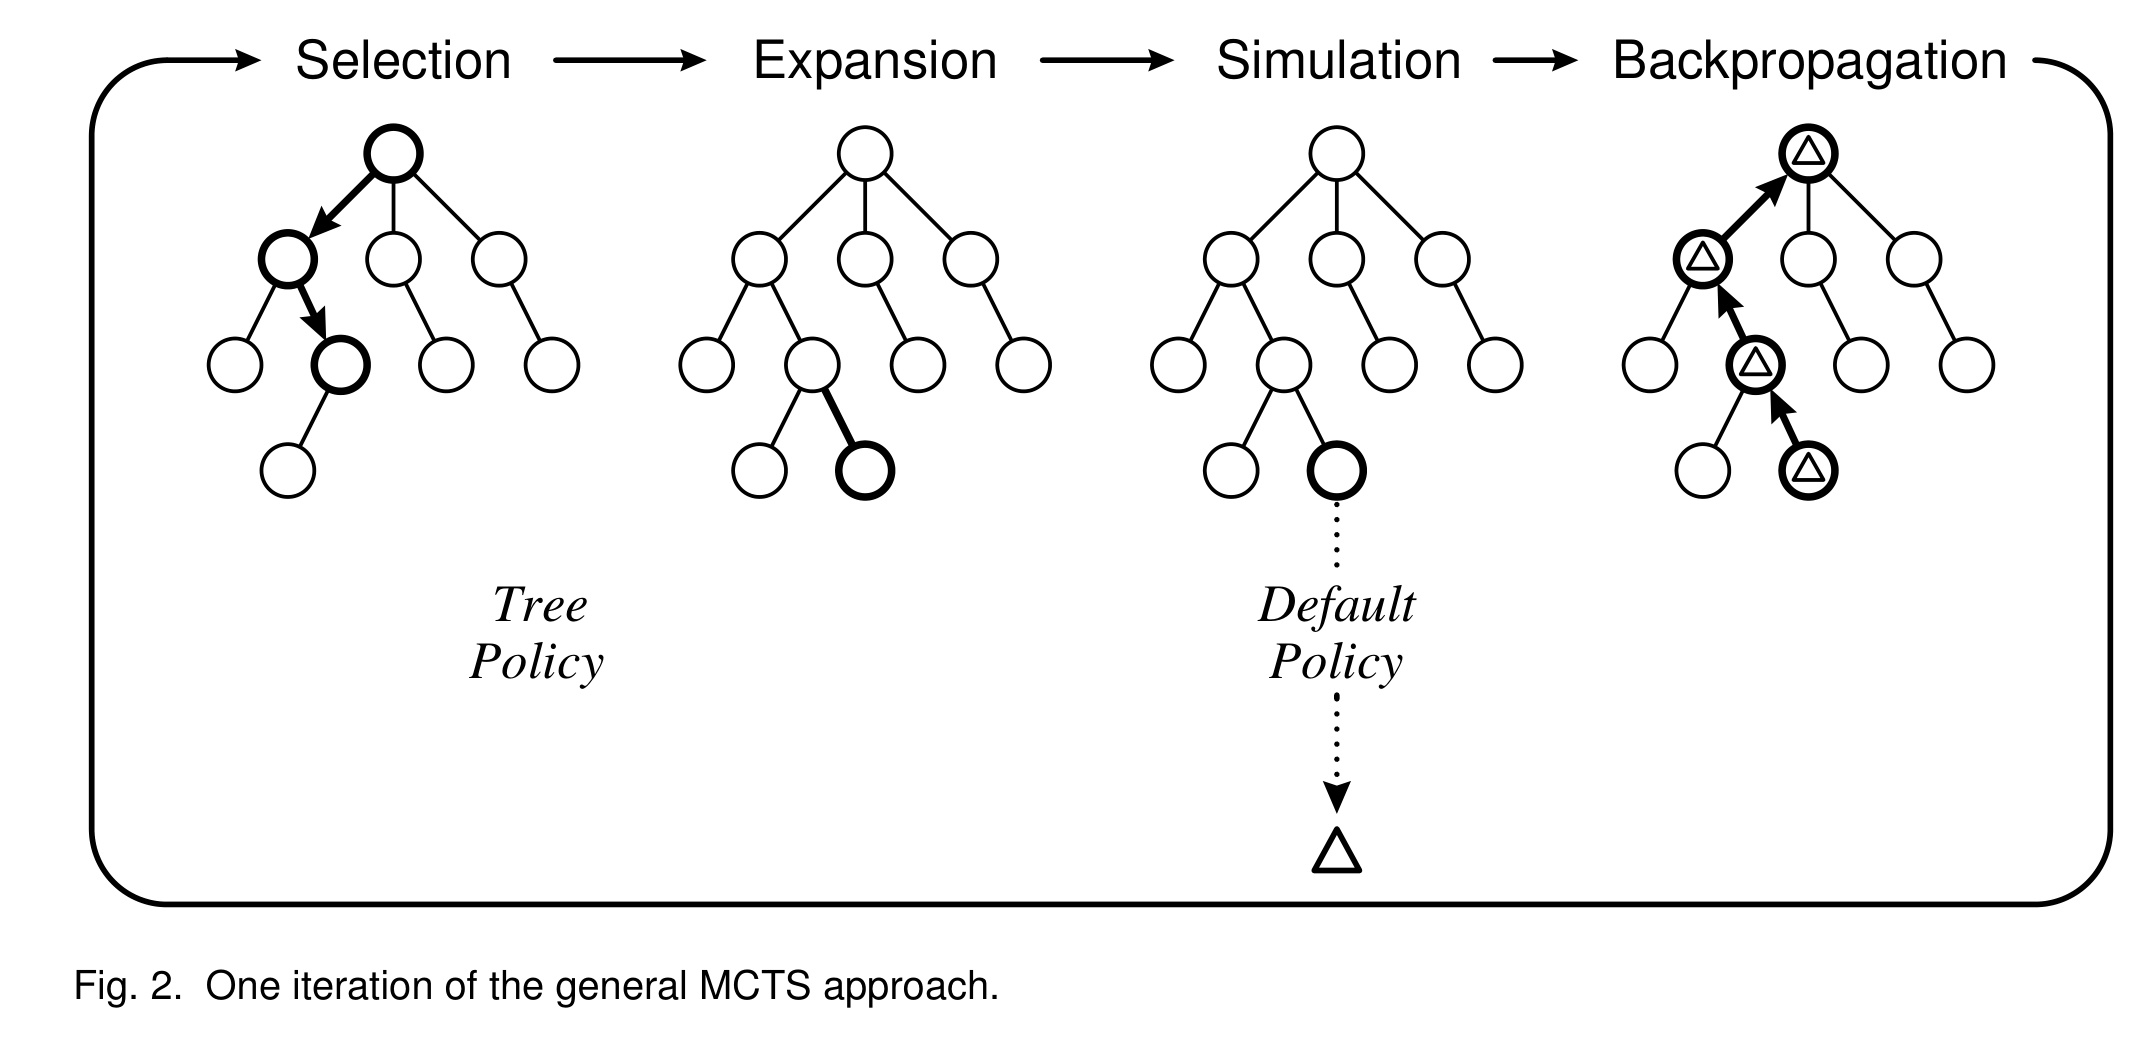
\includegraphics[height=7cm]{\pathroot/theory/reinforcement_learning/images/mcts_approach.jpg}
    \label{fig:mcts_approach}
\end{figure}



\end{enumerate}

上面描述的是UCT (UCB for Tree)算法,可以说是最经典的蒙特卡罗树搜索算法了。
但随着算法的发展,MCTS已经有了非常大的改变。
例如很多围棋AI都已经不再使用纯粹的UCB公式而改用效果更好的UCB1-Tuned了,而搜索方法上也有了非常多的改动了。

Reference:
\begin{itemize}
\item Browne C B, Powley E, Whitehouse D, et al. A Survey of Monte Carlo Tree Search Methods[J]. IEEE Transactions on Computational Intelligence \& Ai in Games, 2012, 4:1(1):1-43.
\item P. Auer, N. Cesa-Bianchi, and P. Fischer, “Finite-time Analysis  of the Multiarmed Bandit Problem,” Mach. Learn., vol. 47, no. 2,  pp. 235-256, 2002.
\end{itemize}

\section{GO}

\url{https://github.com/ardanlabs/gotraining}

\href{https://www.tastehit.com/blog/google-deepmind-alphago-how-it-works/}{Google DeepMind's AlphaGo: How it works}

\href{http://gopherdata.io/post/build_ml_powered_game_ai_tensorflow/}{Building an ML-Powered Game AI using TensorFlow in Go}

\href{https://github.com/TheDuck314/go-NN}{Go-playing neural network in Python using TensorFlow}

\begin{itemize}
\item \href{https://arxiv.org/pdf/1704.03732.pdf}{Learning from Demonstrations for Real World Reinforcement Learning}
\item \href{https://arxiv.org/abs/1312.5602}{Playing Atari with Deep Reinforcement Learning}
\item \href{https://www.intelnervana.com/demystifying-deep-reinforcement-learning/}{Guest Post (Part I): Demystifying Deep Reinforcement Learning}
\item \href{https://storage.googleapis.com/deepmind-media/dqn/DQNNaturePaper.pdf}{Human-level control through deep reinforcement learning}
\item \href{http://simplecore-dev.intel.com/nervana/wp-content/uploads/sites/55/2015/12/ProofQlearning.pdf}{Convergence of Q-learning: a simple proof}
\end{itemize}

$<s, a, r, s'>$

\subsection{贝尔曼方程(Bellman Equation)}
\href{https://zhuanlan.zhihu.com/p/21340755?refer=intelligentunit}{DQN 从入门到放弃3 价值函数与Bellman方程}

\subsection{bandit老虎机}
多臂老虎机




\ifx\mlbook\undefined
    \end{document}
\fi
